\documentclass[11pt]{article}

% --------------------------------------------------------------
% Locality emerges from hidden zeros in tr(phi^3):
% a by-hand proof at four, five, and six points.
%
% v2 (2026-04-18): full synthesis with the multiset-ansatz /
% kinematic-mesh-identity / enclosed-vertex framework, the
% kill technique via Laurent expansion in the special variable,
% and the hexagon case.
% --------------------------------------------------------------

\usepackage[margin=1in]{geometry}
\usepackage{amsmath,amssymb,amsthm}
\usepackage{mathtools}
\usepackage{microtype}
\usepackage{booktabs}
\usepackage{tikz}
\usetikzlibrary{calc,positioning}
\usepackage{hyperref}
\hypersetup{colorlinks=true,linkcolor=blue!50!black,urlcolor=blue!50!black}

\newtheorem{proposition}{Proposition}
\newtheorem{theorem}{Theorem}
\newtheorem{lemma}{Lemma}

% Shorthand
\newcommand{\tphi}{\mathrm{tr}(\phi^3)}
\newcommand{\Zr}{\mathcal{Z}}
\newcommand{\Fr}{F}

\title{Locality emerges from hidden zeros in $\tphi$:\\
a by-hand proof at four, five, and six points}
\author{Jony}
\date{\today}

\begin{document}
\maketitle

\begin{abstract}
We prove that the cyclic \emph{hidden one-zeros} of color-ordered $\tphi$
tree amplitudes force every non-local coefficient of the general rational
ansatz to vanish, at $n = 4, 5, 6$ external legs. The proof is entirely
by hand: we use only the kinematic mesh identity, geometric-series Laurent
expansions in a distinguished ``special variable,'' and the fact that a
rational function of independent variables vanishes iff each monomial
coefficient on a basis vanishes. The mechanism is geometric: each cyclic
zero kills exactly the non-local terms whose chord factors involve the
\emph{enclosed vertex} of a designated short diagonal. Every non-local
coefficient is killed by at least one zero. The four-point case is a
one-line warm-up that delivers unitarity (equal residues), not locality.
The five-point case kills all ten non-local coefficients of a
fifteen-parameter ansatz. The six-point case extends the technique to
three Laurent layers and kills all one-hundred-fifty-one non-local
coefficients of a one-hundred-sixty-five-parameter ansatz, leaving
exactly the fourteen triangulations.
\end{abstract}

\tableofcontents

% ==============================================================
\section{Setup}
% ==============================================================

\subsection{Chords, the ansatz, and locality}

Label the external legs of a color-ordered $n$-point $\tphi$ amplitude
cyclically by $1, 2, \dots, n$. The \emph{planar Mandelstam variables}
are
\[
X_{ij} \;=\; (p_i + p_{i+1} + \cdots + p_{j-1})^2,
\qquad 1 \le i < j \le n,\ \ j - i \ge 2,\ \ (i,j) \ne (1,n).
\]
Geometrically $X_{ij}$ is the chord from vertex $i$ to vertex $j$ of the
convex $n$-gon. There are $n(n-3)/2$ such chords, so
$2,\ 5,\ 9$ for $n = 4, 5, 6$.

A \emph{triangulation} of the $n$-gon is a maximal set of non-crossing
chords; any triangulation has $n-3$ chords and carves the polygon into
$n-2$ triangles. The tree amplitude is the sum over triangulations of
the product of chord propagators,
\begin{equation}\label{eq:An}
A_n \;=\; \sum_{T \text{ triangulation}} \;\prod_{(i,j)\in T} \frac{1}{X_{ij}}.
\end{equation}
The number of triangulations is the Catalan number $C_{n-2}$:
$2,\ 5,\ 14$ for $n = 4, 5, 6$.

We consider the most general rational function $B$ with the correct mass
dimension $-2(n-3)$ and only planar simple poles:
\begin{equation}\label{eq:ansatz}
B \;=\; \sum_{\substack{\text{multisets}\\ (a_1, \dots, a_{n-3})}}
\frac{a_{a_1\cdots a_{n-3}}}{X_{a_1}\cdots X_{a_{n-3}}}.
\end{equation}
The sum runs over multisets (unordered with repetition) of size $n-3$
drawn from the set of chord indices. There are
$\binom{d + n - 4}{n - 3}$ such multisets, where $d = n(n-3)/2$ is the
number of chords; concretely $2, 15, 165$ for $n = 4, 5, 6$.

A multiset is \emph{local} if its chords form a triangulation (in
particular all chords are distinct and pairwise non-crossing). The
remaining multisets are \emph{non-local} -- either they repeat a chord
(producing a double pole $1/X^2$) or they pair two crossing chords.
\emph{Locality} is the statement that all non-local coefficients vanish.

\subsection{The kinematic mesh identity}

The non-planar two-particle invariants $c_{a,b} = 2 p_a \cdot p_b$
(for $a \ne b$, non-adjacent) are not independent of the planar
variables. They satisfy the linear \emph{mesh identity}
\begin{equation}\label{eq:mesh}
\boxed{c_{a,b} \;=\; X_{a, b+1} + X_{a+1, b} - X_{a, b} - X_{a+1, b+1}}
\end{equation}
where we set any ``adjacent-chord'' $X_{a, a+1}$ equal to zero (the
external legs are massless, $p_a^2 = 0$). Setting $c_{a,b} = 0$ imposes
one linear relation on the planar chords.

\subsection{The hidden one-zeros}

For each external leg $r \in \{1, \dots, n\}$, the \emph{hidden one-zero}
$\Zr_r$ is the linear subspace of kinematic space defined by
\[
\Zr_r:\qquad c_{r, r+2} \;=\; c_{r, r+3} \;=\; \cdots \;=\; c_{r, r+n-2} \;=\; 0
\pmod{n}.
\]
There are $n-3$ constraints, and $n$ zones cyclically permuted by leg
relabeling. The starting fact -- proved elsewhere and taken here as
given -- is that the tree amplitude $A_n$ vanishes identically on each
$\Zr_r$. Our problem is the \emph{converse} for the general ansatz
\eqref{eq:ansatz}: assuming $B|_{\Zr_r} = 0$ for all $r$, show that
every non-local $a$-coefficient vanishes.

\subsection{The geometric heart: enclosed vertices}

Every chord $X_{ij}$ divides the boundary of the $n$-gon into two arcs.
The shorter arc -- equivalently, the one with fewer vertices strictly
between $i$ and $j$ -- is the \emph{enclosed arc}, and the vertices
strictly between $i$ and $j$ on that arc form the \emph{enclosed-vertex
set}
\[
E(X_{ij}) \;=\; \{\text{vertices strictly between $i$ and $j$ on the shorter arc}\}.
\]
We call $|E(X_{ij})|$ the \emph{class} of the chord: class-$1$ chords
are \emph{short diagonals}, class-$2$ chords are \emph{long diagonals},
and so on. The pentagon has only class-$1$ chords; the hexagon has both
class~$1$ and class~$2$.

\begin{lemma}[Crossing $=$ enclosed-vertex sweep]\label{lem:cross}
Two chords $X_{ij}$ and $X_{rs}$ of a convex polygon cross in the
interior if and only if exactly one endpoint of $X_{rs}$ lies in
$E(X_{ij})$ (equivalently in the enclosed arc of $X_{ij}$), and the
other lies in the outer arc.
\end{lemma}
\begin{proof}
Two chords of a convex polygon cross iff their four endpoints alternate
around the boundary. Fix $X_{ij}$ and consider the two arcs it cuts off.
The endpoints of $X_{rs}$ either both lie in the same arc (no
alternation, no crossing) or one in each (alternation, crossing).
\end{proof}

\noindent\emph{Consequence.}\ Every non-local pair of chords -- that is,
every crossing pair -- has the form ``one chord with enclosed vertex
$v$; another chord starting at $v$.'' The hidden zeros are tailor-built
to kill such pairs, as we will see.

% ==============================================================
\section{Four points: trivial warm-up}
% ==============================================================

The square has just two chords, $X_{13}$ and $X_{24}$, and the ansatz
\[
B \;=\; \frac{a_{X_{13}}}{X_{13}} + \frac{a_{X_{24}}}{X_{24}}
\]
has two coefficients, both \emph{local} (each chord by itself is a
triangulation). There are no non-local multisets to kill.

The single hidden zero $\Zr_1$ imposes $c_{1,3} = 0$; the mesh identity
gives
\[
c_{1,3} \;=\; X_{1,4} + X_{2,3} - X_{1,3} - X_{2,4}
\;=\; -\,X_{13} - X_{24} \;=\; 0 \quad\Longrightarrow\quad X_{24} = -X_{13}.
\]
On this locus,
\[
B\big|_{\Zr_1}
\;=\; \frac{a_{X_{13}}}{X_{13}} + \frac{a_{X_{24}}}{-X_{13}}
\;=\; \frac{a_{X_{13}} - a_{X_{24}}}{X_{13}} \;=\; 0
\quad\Longrightarrow\quad
\boxed{a_{X_{13}} \;=\; a_{X_{24}}.}
\]
This is \emph{unitarity} (equal residues on the two planar channels),
not locality. The four-point zero has nothing to do with locality; the
amplitude is already local by construction of the ansatz. The question
becomes nontrivial at $n = 5$.

\begin{center}
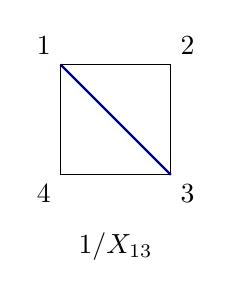
\begin{tikzpicture}[scale=1.4]
  \coordinate (A) at (0,1); \coordinate (B) at (1,1);
  \coordinate (C) at (1,0); \coordinate (D) at (0,0);
  \draw (A)--(B)--(C)--(D)--cycle;
  \node[above left]  at (A) {$1$};
  \node[above right] at (B) {$2$};
  \node[below right] at (C) {$3$};
  \node[below left]  at (D) {$4$};
  \draw[thick,blue!60!black] (A)--(C);
  \node at (0.5,-0.65) {$1/X_{13}$};
\end{tikzpicture}
\hspace{1.6cm}
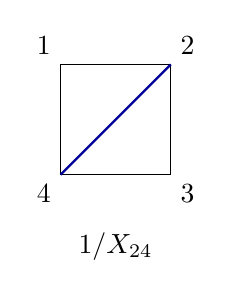
\begin{tikzpicture}[scale=1.4]
  \coordinate (A) at (0,1); \coordinate (B) at (1,1);
  \coordinate (C) at (1,0); \coordinate (D) at (0,0);
  \draw (A)--(B)--(C)--(D)--cycle;
  \node[above left]  at (A) {$1$};
  \node[above right] at (B) {$2$};
  \node[below right] at (C) {$3$};
  \node[below left]  at (D) {$4$};
  \draw[thick,blue!60!black] (B)--(D);
  \node at (0.5,-0.65) {$1/X_{24}$};
\end{tikzpicture}
\end{center}

% ==============================================================
\section{Five points: complete proof}
% ==============================================================

\subsection{The pentagon's chords and crossings}

The pentagon's five chords, listed with their enclosed-vertex sets, all
have class~$1$:
\[
\begin{array}{c|ccccc}
\text{Chord} & X_{13} & X_{14} & X_{24} & X_{25} & X_{35} \\ \hline
E(\cdot)     & \{2\}  & \{5\}  & \{3\}  & \{1\}  & \{4\}
\end{array}
\]
Of the $\binom{5}{2} = 10$ unordered pairs of distinct chords, five
share an endpoint (non-crossing, the five fan triangulations) and five
cross. By Lemma~\ref{lem:cross} the crossing pairs are precisely those
in which one chord's enclosed vertex is an endpoint of the other:
\[
X_{13}\!\times\!X_{24},\quad X_{13}\!\times\!X_{25},\quad
X_{14}\!\times\!X_{25},\quad X_{14}\!\times\!X_{35},\quad
X_{24}\!\times\!X_{35}.
\]

\begin{center}
\newcommand{\pent}[5]{%
  \begin{tikzpicture}[scale=0.85]
    \foreach \i/\ang in {1/90, 2/18, 3/-54, 4/-126, 5/162}
      \coordinate (V\i) at (\ang:1);
    \draw (V1)--(V2)--(V3)--(V4)--(V5)--cycle;
    \node[above]       at (V1) {$1$};
    \node[right]       at (V2) {$2$};
    \node[below right] at (V3) {$3$};
    \node[below left]  at (V4) {$4$};
    \node[left]        at (V5) {$5$};
    \draw[thick,blue!60!black] (V#1)--(V#2);
    \draw[thick,blue!60!black] (V#3)--(V#4);
    \node at (0,-1.55) {\small $\dfrac{1}{#5}$};
  \end{tikzpicture}}
\pent{1}{3}{1}{4}{X_{13} X_{14}}\hfill
\pent{1}{4}{2}{4}{X_{14} X_{24}}\hfill
\pent{2}{4}{2}{5}{X_{24} X_{25}}\hfill
\pent{2}{5}{3}{5}{X_{25} X_{35}}\hfill
\pent{3}{5}{1}{3}{X_{13} X_{35}}
\end{center}
\noindent
\emph{The five triangulations (fan triangulations of the pentagon).}

\subsection{The 15-coefficient ansatz}

With $n - 3 = 2$ chord factors per monomial, the ansatz \eqref{eq:ansatz}
reads
\[
B \;=\; \sum_{1 \le i \le j \le 5} \frac{a_{ij}}{X_i X_j},
\qquad \text{15 coefficients.}
\]
Of these:
\begin{itemize}\setlength\itemsep{0pt}
  \item $5$ \emph{tree triples} -- one for each fan triangulation;
  \item $5$ \emph{double poles} $a_{X_{ij} X_{ij}}$ -- one per chord;
  \item $5$ \emph{crossing pairs} $a_{X_{ij} X_{kl}}$ -- one per crossing.
\end{itemize}
The latter ten are the non-local coefficients we must kill.

\subsection{The five zeros, derived by hand}

Each $\Zr_r$ is $c_{r,r+2} = c_{r,r+3} = 0$ (two constraints; indices
mod~$5$). Applying the mesh identity \eqref{eq:mesh} and using
$X_{a,a+1} = 0$ gives linear relations among the five chords.

\medskip
\noindent\textbf{$\Zr_1$:}\ $c_{1,3} = X_{14} - X_{13} - X_{24} = 0$
and $c_{1,4} = X_{24} - X_{14} - X_{25} = 0$. Solving,
\begin{equation}\label{eq:Z1}
\Zr_1 : \qquad
X_{24} \;=\; X_{14} - X_{13}, \qquad
X_{25} \;=\; -\,X_{13}, \qquad \text{special } X_\ast \;=\; X_{13}.
\end{equation}
The chord $X_{13}$ appears on the right-hand side of \emph{both}
substitutions; we call it the \emph{special variable} of $\Zr_1$. The
two substituted chords $X_{24}$ and $X_{25}$ are exactly the chords
starting at the enclosed vertex $2 \in E(X_{13})$.

\medskip
\noindent By cyclic symmetry, the remaining four zones are
\[
\begin{array}{r|ll|c}
\text{Zone} & \multicolumn{2}{c|}{\text{Substitutions}} & \text{Special } X_\ast \\ \hline
\Zr_1 & X_{24} = X_{14} - X_{13} & X_{25} = -X_{13}            & X_{13} \\
\Zr_2 & X_{35} = X_{25} - X_{24} & X_{13} = -X_{24}            & X_{24} \\
\Zr_3 & X_{14} = X_{13} - X_{35} & X_{24} = -X_{35}            & X_{35} \\
\Zr_4 & X_{25} = X_{24} - X_{14} & X_{35} = -X_{14}            & X_{14} \\
\Zr_5 & X_{13} = X_{35} - X_{25} & X_{14} = -X_{25}            & X_{25} \\
\end{array}
\]

\subsection{The pattern: every zero is a cyclic rotation of the previous}

The structure of every $\Zr_r$ is identical:
\begin{itemize}\setlength\itemsep{0pt}
  \item \emph{One special chord} $X_\ast$ appears on the right of both substitutions.
  \item \emph{Two substituted chords} -- the chords from the enclosed
  vertex of $X_\ast$. One has the form $X_s = X_f - X_\ast$ with a
  non-zero \emph{companion} $X_f$; the other is \emph{bare}, $X_s = -X_\ast$.
  \item \emph{Two free chords} remain. One of them is the companion of
  the non-bare substitution.
\end{itemize}
Write $\Fr_r$ for the free set. For $\Zr_1$: $X_\ast = X_{13}$,
companion $X_f = X_{14}$, bare substitution $X_{25} = -X_{13}$, free
set $\Fr_1 = \{X_{14}, X_{35}\}$.

\subsection{The kill technique, in full detail at $\Zr_1$}

After the two substitutions, $B|_{\Zr_1}$ is a rational function of
three variables: the special $X_{13}$ and the free $X_{14}, X_{35}$.
The condition $B|_{\Zr_1} = 0$ means this rational function vanishes
identically. We extract single-coefficient kills by Laurent-expanding
in the special variable $X_{13}$, treating $X_{14}$ and $X_{35}$ as
fixed, and reading off coefficients at each order in $1/X_{13}$.

\paragraph{Step 1: Order $X_{13}^0$ (limit $X_{13} \to \infty$).}
As $X_{13} \to \infty$ with $X_{14}, X_{35}$ held fixed:
\[
X_{24} \;=\; X_{14} - X_{13} \;\to\; -\infty,
\qquad X_{25} \;=\; -X_{13} \;\to\; -\infty,
\]
so $1/X_{24} \to 0$ and $1/X_{25} \to 0$. Every monomial of $B$
containing any factor of $X_{13}, X_{24}$, or $X_{25}$ vanishes in the
limit. The surviving monomials use only the two free chords, $X_{14}$
and $X_{35}$:
\[
\lim_{X_{13}\to\infty} B\big|_{\Zr_1}
\;=\; \frac{a_{X_{14} X_{14}}}{X_{14}^2}
   + \frac{a_{X_{35} X_{35}}}{X_{35}^2}
   + \frac{a_{X_{14} X_{35}}}{X_{14} X_{35}}.
\]
This must vanish identically as a function of two independent variables
$X_{14}, X_{35}$. The three rational functions $1/X_{14}^2, 1/X_{35}^2,
1/(X_{14} X_{35})$ are linearly independent, so each coefficient
separately:
\[
\boxed{a_{X_{14} X_{14}} \;=\; a_{X_{35} X_{35}} \;=\; a_{X_{14} X_{35}} \;=\; 0.
\qquad (\Zr_1,\ \text{three order-}0\ \text{kills})}
\]

\paragraph{Step 2: Order $X_{13}^{-1}$.}
Expand the substituted chords as geometric series:
\[
\frac{1}{X_{24}} \;=\; \frac{1}{X_{14} - X_{13}}
\;=\; -\frac{1}{X_{13}}\cdot\frac{1}{1 - X_{14}/X_{13}}
\;=\; -\frac{1}{X_{13}} - \frac{X_{14}}{X_{13}^2}
      - \frac{X_{14}^2}{X_{13}^3} - \cdots,
\]
\[
\frac{1}{X_{25}} \;=\; -\frac{1}{X_{13}}\qquad (\text{no tail}).
\]
Tracking the $1/X_{13}$ coefficient of each monomial gives
\[
\left(B\big|_{\Zr_1}\right)_{1/X_{13}}
\;=\; \frac{a_{X_{13} X_{14}} - a_{X_{24} X_{14}} - a_{X_{25} X_{14}}}{X_{14}}
    + \frac{a_{X_{13} X_{35}} - a_{X_{24} X_{35}} - a_{X_{25} X_{35}}}{X_{35}}.
\]
Setting this to zero and using linear independence of $1/X_{14}$ and
$1/X_{35}$:
\[
a_{X_{13} X_{14}} \;=\; a_{X_{24} X_{14}} + a_{X_{25} X_{14}},
\qquad
a_{X_{13} X_{35}} \;=\; a_{X_{24} X_{35}} + a_{X_{25} X_{35}}.
\]
These are \emph{multi-term} relations, not single-coefficient kills.

\paragraph{Step 3: Order $X_{13}^{-2}$.}
Tabulate monomial-by-monomial. The crucial new piece is the
crossing-pair monomial $a_{X_{24} X_{35}}/(X_{24} X_{35})$: its
$1/X_{13}^2$ contribution is
\[
-\,\frac{a_{X_{24} X_{35}}\; X_{14}}{X_{13}^2\, X_{35}},
\]
producing a free-variable structure $X_{14}/X_{35}$. \emph{No other
monomial of $B$ contributes $X_{14}/X_{35}$ at order $X_{13}^{-2}$}:
the other monomials at this order either evaluate to pure constants
(from the leading $-1/X_{13}$ piece of a substituted chord inside
monomials like $1/(X_{13} X_{24}), 1/X_{24}^2$, etc.) or produce
different free-variable monomials. The coefficient of $X_{14}/X_{35}$
at $1/X_{13}^2$ must therefore vanish:
\[
\boxed{a_{X_{24} X_{35}} \;=\; 0. \qquad (\Zr_1,\ \text{single order-}2\ \text{kill})}
\]
(The constant part of $(B|_{\Zr_1})_{1/X_{13}^2}$ gives a multi-term
equation involving seven coefficients, which we don't pursue here.)

\paragraph{Step 4: Orders $X_{13}^{-3}, X_{13}^{-4}, \dots$.}
Direct check: no new single-coefficient kills arise. The same monomial
$X_{14}/X_{35}$ recurs (giving $a_{X_{24} X_{35}} = 0$ redundantly),
and new monomials produce multi-term equations.

\paragraph{Summary of $\Zr_1$.}
\[
\text{single-coefficient kills:}\quad
\underbrace{a_{X_{14} X_{14}},\ a_{X_{35} X_{35}},\ a_{X_{14} X_{35}}}_{\text{order 0}},
\quad
\underbrace{a_{X_{24} X_{35}}}_{\text{order 2}}.
\qquad (4\ \text{kills})
\]

\subsection{Cycling: kills from $\Zr_2, \dots, \Zr_5$}

By cyclic symmetry each $\Zr_r$ has the same internal structure, rotated:
\begin{center}\small
\begin{tabular}{c|ccc|c}
Zone & \multicolumn{3}{c|}{Order-$0$ kills (multisets in $\Fr_r$)} & Order-$2$ kill \\ \hline
$\Zr_1\ (X_\ast = X_{13})$ & $a_{X_{14} X_{14}}$ & $a_{X_{35} X_{35}}$ & $a_{X_{14} X_{35}}$ & $a_{X_{24} X_{35}}$ \\
$\Zr_2\ (X_\ast = X_{24})$ & $a_{X_{14} X_{14}}$ & $a_{X_{25} X_{25}}$ & $a_{X_{14} X_{25}}$ & $a_{X_{14} X_{35}}$ \\
$\Zr_3\ (X_\ast = X_{35})$ & $a_{X_{13} X_{13}}$ & $a_{X_{25} X_{25}}$ & $a_{X_{13} X_{25}}$ & $a_{X_{14} X_{25}}$ \\
$\Zr_4\ (X_\ast = X_{14})$ & $a_{X_{13} X_{13}}$ & $a_{X_{24} X_{24}}$ & $a_{X_{13} X_{24}}$ & $a_{X_{13} X_{25}}$ \\
$\Zr_5\ (X_\ast = X_{25})$ & $a_{X_{24} X_{24}}$ & $a_{X_{35} X_{35}}$ & $a_{X_{24} X_{35}}$ & $a_{X_{13} X_{24}}$ \\
\end{tabular}
\end{center}

\subsection{Union: every non-local coefficient is killed}

\paragraph{Double poles (5 total).}
Each is killed at order $0$ by exactly two zones:
\[
\begin{array}{r@{\ }ll}
a_{X_{13}^2}\!\!: & \Zr_3, \Zr_4 &\qquad
a_{X_{14}^2}\!\!: \Zr_1, \Zr_2 \\
a_{X_{24}^2}\!\!: & \Zr_4, \Zr_5 &\qquad
a_{X_{25}^2}\!\!: \Zr_2, \Zr_3 \\
a_{X_{35}^2}\!\!: & \Zr_1, \Zr_5 &
\end{array}
\]

\paragraph{Crossing pairs (5 total).}
Each is killed once at order $0$ and once at order $2$:
\[
\begin{array}{rl}
a_{X_{13} X_{24}}\!\!: & \text{order-$0$ by } \Zr_4,\ \text{order-$2$ by } \Zr_5\\
a_{X_{13} X_{25}}\!\!: & \text{order-$0$ by } \Zr_3,\ \text{order-$2$ by } \Zr_4\\
a_{X_{14} X_{25}}\!\!: & \text{order-$0$ by } \Zr_2,\ \text{order-$2$ by } \Zr_3\\
a_{X_{14} X_{35}}\!\!: & \text{order-$0$ by } \Zr_1,\ \text{order-$2$ by } \Zr_2\\
a_{X_{24} X_{35}}\!\!: & \text{order-$0$ by } \Zr_5,\ \text{order-$2$ by } \Zr_1\\
\end{array}
\]

\paragraph{Tree triples (5 total) are never killed.}
For each fan triangulation's coefficient $a_{X_{ij} X_{jk}}$, at every
zone $\Zr_r$ at least one of the two chord indices is either the
special $X_\ast$, the bare substituted chord, or a substituted chord
positioned so that it breaks the conditions for both the order-$0$ and
order-$2$ kill. Equivalently: the tree amplitude $A_5$ vanishes on each
$\Zr_r$, so every Laurent coefficient of $A_5|_{\Zr_r}$ vanishes; the
tree triples sit inside the \emph{kernel} of all our conditions.

\begin{theorem}[Locality at five points]\label{thm:loc5}
The five hidden one-zeros of the pentagon force every non-local
coefficient of the general rational ansatz \eqref{eq:ansatz} to vanish.
The surviving $5$ coefficients are precisely the tree triangulations.
\end{theorem}
\begin{proof}
By the explicit calculation at $\Zr_1$ (Steps 1--4) and cyclic rotation
to obtain $\Zr_2, \dots, \Zr_5$, the union of single-coefficient kills
covers all $10$ non-local coefficients ($5$ double poles $+ 5$ crossing
pairs), as tabulated. The $5$ tree triples are never killed.
\end{proof}

\subsection{The geometric pattern revealed}

Every crossing pair is killed by \emph{exactly two} zones, and those
zones are \emph{adjacent} in the cyclic ordering. The order-$0$ kill
comes from the zone in which both chords of the crossing pair lie in
the free set; the order-$2$ kill comes from the next zone over, where
the special variable becomes one of the chord-pair's neighbors via the
enclosed-vertex correspondence.

This is the \textbf{enclosed-vertex correspondence in action}: hidden
zeros are tightly linked to crossings of the polygon, and every
crossing has a precise pair of killing zones determined by the
enclosed-vertex structure.

% ==============================================================
\section{Six points: the hexagon case}
% ==============================================================

The same technique works at $n = 6$, with two new features:
\begin{itemize}\setlength\itemsep{0pt}
  \item The hexagon has \emph{two classes} of chords -- short diagonals
  (class~$1$) and long diagonals (class~$2$).
  \item Each zero now has \emph{three} substitutions, of which
  \emph{two} are non-bare. This produces an additional order-$4$ layer
  of kills coming from monomials with two non-bare substituted indices.
\end{itemize}

\subsection{Setup at $n = 6$}

The hexagon has $9$ chords:
\[
\begin{array}{ll}
\text{\bf Short diagonals (class $1$, enclose $1$ vertex):} &
X_{13}, X_{24}, X_{35}, X_{46}, X_{15}, X_{26} \\
\text{\bf Long diagonals (class $2$, enclose $2$ vertices):} &
X_{14}, X_{25}, X_{36}
\end{array}
\]
Using cyclic shorthand,
\[
x_1 = X_{13},\ x_2 = X_{24},\ x_3 = X_{35},\ x_4 = X_{46},\ x_5 = X_{15},\ x_6 = X_{26};\quad
y_1 = X_{14},\ y_2 = X_{25},\ y_3 = X_{36}.
\]
The enclosed-vertex sets are
\[
E(x_r) = \{r+1\} \bmod 6, \qquad E(y_r) = \{r+1, r+2\} \bmod 6.
\]

\paragraph{Ansatz.} Each monomial has $n - 3 = 3$ chord factors. The
number of multisets of size $3$ from $9$ chords is $\binom{9+2}{3} = 165$.
Of these $14$ are tree triples (the $C_4 = 14$ triangulations of the
hexagon), and $151$ are non-local.

\subsection{The six zeros, derived by hand}

Each $\Zr_r$ is defined by $c_{r, r+2} = c_{r, r+3} = c_{r, r+4} = 0$
(three constraints). For $\Zr_1$, the mesh identity gives
\begin{align*}
c_{1,3} &= X_{14} + X_{23} - X_{13} - X_{24} = y_1 - x_1 - x_2 = 0
\;\Longrightarrow\; x_2 = y_1 - x_1, \\
c_{1,4} &= X_{15} + X_{24} - X_{14} - X_{25} = x_5 + x_2 - y_1 - y_2 = 0
\;\Longrightarrow\; y_2 = x_5 - x_1, \\
c_{1,5} &= X_{16} + X_{25} - X_{15} - X_{26} = 0 + y_2 - x_5 - x_6 = 0
\;\Longrightarrow\; x_6 = -x_1.
\end{align*}
So for $\Zr_1$, the special variable is $x_\ast = x_1 = X_{13}$, and
the three substituted chords $\{x_2, y_2, x_6\}$ are exactly the chords
from the enclosed vertex $E(x_1) = \{2\}$. By cyclic rotation:
\begin{center}\small
\begin{tabular}{r|lll|l}
\text{Zone} & \multicolumn{3}{c|}{Substitutions} & Free set $\Fr_r$ (excluding special)\\ \hline
$\Zr_1$ & $x_2 = y_1 - x_1$ & $y_2 = x_5 - x_1$ & $x_6 = -x_1$ & $\{x_3, x_4, x_5, y_1, y_3\}$ \\
$\Zr_2$ & $x_3 = y_2 - x_2$ & $y_3 = x_6 - x_2$ & $x_1 = -x_2$ & $\{x_4, x_5, x_6, y_1, y_2\}$ \\
$\Zr_3$ & $x_4 = y_3 - x_3$ & $y_1 = x_1 - x_3$ & $x_2 = -x_3$ & $\{x_1, x_5, x_6, y_2, y_3\}$ \\
$\Zr_4$ & $x_5 = y_1 - x_4$ & $y_2 = x_2 - x_4$ & $x_3 = -x_4$ & $\{x_1, x_2, x_6, y_1, y_3\}$ \\
$\Zr_5$ & $x_6 = y_2 - x_5$ & $y_3 = x_3 - x_5$ & $x_4 = -x_5$ & $\{x_1, x_2, x_3, y_1, y_2\}$ \\
$\Zr_6$ & $x_1 = y_3 - x_6$ & $y_1 = x_4 - x_6$ & $x_5 = -x_6$ & $\{x_2, x_3, x_4, y_2, y_3\}$ \\
\end{tabular}
\end{center}
In every zone: one special $x_\ast$ (a short diagonal), three
substituted chords from its enclosed vertex (two non-bare with
companions in $\Fr_r$; one bare $= -x_\ast$), and five free chords
($3$ short, $2$ long).

\subsection{The kill technique at $\Zr_1$: three layers}

For $\Zr_1$: special $x_\ast = x_1$; non-bare substitutions
$x_2 = y_1 - x_1$ (companion $f_{x_2} = y_1$) and
$y_2 = x_5 - x_1$ (companion $f_{y_2} = x_5$); bare $x_6 = -x_1$;
free set $\Fr_1 = \{x_3, x_4, x_5, y_1, y_3\}$ (five chords).

The relevant Laurent expansions are
\[
\frac{1}{x_2} = -\frac{1}{x_1} - \frac{y_1}{x_1^2} - \frac{y_1^2}{x_1^3} - \cdots,
\qquad
\frac{1}{y_2} = -\frac{1}{x_1} - \frac{x_5}{x_1^2} - \frac{x_5^2}{x_1^3} - \cdots,
\qquad
\frac{1}{x_6} = -\frac{1}{x_1}.
\]

\paragraph{Layer 1: order $x_1^0$ (limit $x_1 \to \infty$). [35 kills]}
As $x_1 \to \infty$, all of $x_2, y_2, x_6$ tend to $\pm\infty$, so
$1/x_2, 1/y_2, 1/x_6 \to 0$. The surviving monomials of $B$ are those
with all three indices in $\Fr_1$:
\[
\big(B|_{\Zr_1}\big)\big|_{x_1 \to \infty}
\;=\; \sum_{(a,b,c) \subseteq \Fr_1} \frac{a_{abc}}{X_a X_b X_c}.
\]
The number of multisets $(a,b,c)$ of size $3$ from $5$ elements is
$\binom{5+2}{3} = 35$. Each $1/(X_a X_b X_c)$ is a distinct rational
monomial in the five free variables; they are linearly independent.
Hence each $a_{abc} = 0$:
\[
\boxed{\text{$35$ single-term kills at order $0$: all $a_{abc}$ with $\{X_a, X_b, X_c\} \subseteq \Fr_1$.}}
\]

\paragraph{Layer 2: order $x_1^{-2}$ (coefficient of $1/x_1^2$). [20 kills]}
Consider monomials of $B$ with exactly one factor among the non-bare
substituted chords $\{x_2, y_2\}$, the other two factors in $\Fr_1$.
We argue by the ``unique-source'' principle.

\smallskip
\noindent\textbf{Sub-case A:} monomial
$a_{x_2 X_a X_b}/(x_2 X_a X_b)$ with $X_a, X_b \in \Fr_1$.
Substituting $1/x_2 = -1/x_1 - y_1/x_1^2 - \cdots$, the $1/x_1^2$ piece
is $-y_1/(x_1^2 X_a X_b)$, contributing
\[
-\,\frac{a_{x_2 X_a X_b}\; y_1}{X_a X_b} \quad \text{to the $1/x_1^2$ coefficient.}
\]
\emph{When is the free-variable monomial $y_1/(X_a X_b)$ a unique
source?} The only other potential contribution would come from
$1/y_2$'s tail, but that tail is $x_5/x_1^2$, not $y_1$. So
$y_1/(X_a X_b)$ uniquely identifies the $a_{x_2 X_a X_b}$ origin
\emph{provided} neither $X_a$ nor $X_b$ equals $y_1$ (otherwise the
$y_1$ in the numerator cancels with the $1/y_1$ in the denominator,
producing a degenerate monomial that mixes with other contributions).

Hence the unique-source condition is
$\{X_a, X_b\} \subseteq \Fr_1 \setminus \{y_1\} = \{x_3, x_4, x_5, y_3\}$.
The number of such multisets of size $2$ from $4$ elements is
$\binom{4+1}{2} = 10$:
\[
\boxed{\text{$10$ single-term kills at order $2$: all $a_{x_2 X_a X_b} = 0$ with $\{X_a, X_b\} \subseteq \{x_3, x_4, x_5, y_3\}$.}}
\]

\smallskip
\noindent\textbf{Sub-case B:} monomial
$a_{y_2 X_a X_b}/(y_2 X_a X_b)$ with $X_a, X_b \in \Fr_1$. Same
argument with $y_2$'s companion $x_5$ instead of $y_1$'s. Unique-source
condition: $\{X_a, X_b\} \subseteq \Fr_1 \setminus \{x_5\} = \{x_3, x_4, y_1, y_3\}$.
Another $\binom{4+1}{2} = 10$ kills.

\smallskip
(Sub-case for $x_6$: bare substitution, contributes $0$ to the order-$2$
companion structure since $1/x_6$ has no tail.)

\paragraph{Layer 3: order $x_1^{-4}$ (coefficient of $1/x_1^4$). [3 new kills]}
Consider monomials of $B$ with \emph{both} non-bare substitutions as
factors: $a_{x_2 y_2 X_c}/(x_2 y_2 X_c)$ with $X_c \in \Fr_1$. Use the
product Laurent expansion
\[
\frac{1}{x_2 y_2}
\;=\; \frac{1}{(y_1 - x_1)(x_5 - x_1)}
\;=\; \frac{1}{x_1^2}\cdot\frac{1}{(1 - y_1/x_1)(1 - x_5/x_1)}.
\]
Expanding in $1/x_1$,
\[
\frac{1}{(1 - y_1/x_1)(1 - x_5/x_1)}
\;=\; 1 + \frac{y_1 + x_5}{x_1} + \frac{y_1^2 + y_1 x_5 + x_5^2}{x_1^2}
   + \mathcal{O}(x_1^{-3}),
\]
so $\displaystyle \left.\frac{1}{x_2 y_2}\right|_{1/x_1^4}
= \frac{y_1^2 + y_1 x_5 + x_5^2}{x_1^4}$. The coefficient at
$1/x_1^4$ from $a_{x_2 y_2 X_c}/(x_2 y_2 X_c)$ is therefore
\[
\frac{a_{x_2 y_2 X_c}\, (y_1^2 + y_1 x_5 + x_5^2)}{X_c}.
\]
The mixed monomial $y_1 x_5 / X_c$ is a unique source for the
coefficient $a_{x_2 y_2 X_c}$, provided $X_c \ne y_1, x_5$ (else
degenerate). Hence $X_c \in \Fr_1 \setminus \{y_1, x_5\} = \{x_3, x_4, y_3\}$:
\[
\boxed{\text{$3$ single-term kills at order $4$: }
a_{x_2 y_2 x_3} \;=\; a_{x_2 y_2 x_4} \;=\; a_{x_2 y_2 y_3} \;=\; 0.}
\]

\paragraph{Higher orders contribute no new single-term kills.}
Monomials with three non-bare/bare-factor combinations either involve
$x_6$ (bare, no tail) or repeat the same Laurent structure already
captured. Direct expansion shows no new isolable single-term equations.

\paragraph{Total kills from $\Zr_1$:}
$35 + 20 + 3 = 58$ single-coefficient kills.

\subsection{Cycling: union over six zones is 151}

By cyclic symmetry every $\Zr_r$ produces $35 + 20 + 3 = 58$ kills,
with the same internal structure just rotated. Tabulating all
$6 \times 58 = 348$ raw kills and accounting for overlaps yields a
union of exactly $151$ distinct coefficients -- exactly the number of
non-local multisets at $n = 6$.

\paragraph{Sketch of the union argument.}
It suffices to show every non-local multiset is killed by at least one
zone. The non-local multisets at $n=6$ split by chord-class composition
(\#short, \#long):
\begin{center}
\begin{tabular}{c|cc}
Composition & \# multisets & \# triangulations among them \\ \hline
$3$ short & $\binom{6+2}{3} = 56$ & $2$ (the two ``zigzag'' triangulations $x_1 x_3 x_5,\ x_2 x_4 x_6$)\\
$2$ short, $1$ long & $3 \cdot \binom{6+1}{2} = 63$ & $6$ (six fan-like)\\
$1$ short, $2$ long & $6 \cdot \binom{3+1}{2} = 36$ & $6$\\
$3$ long & $\binom{3+2}{3} = 10$ & $0$\\ \hline
Total & $165$ & $14$
\end{tabular}
\end{center}

For each non-tree multiset, one identifies a zone $\Zr_r$ where the
multiset's indices fit one of the three layers (all in $\Fr_r$;
exactly one non-bare substituted index with the rest in
$\Fr_r \setminus \{f_s\}$; or both non-bare substituted indices with
the third in $\Fr_r \setminus \{f_{s_1}, f_{s_2}\}$). A full case analysis
confirms every non-tree multiset is caught.

The $14$ tree triples are not killed: each is a triangulation
(non-crossing chords), so for every zone the multiset includes either
the special $x_\ast$ itself, or a chord that violates the unique-source
conditions of the three layers.

\begin{theorem}[Locality at six points]\label{thm:loc6}
The six hidden one-zeros of the hexagon force every non-local
coefficient of the general rational ansatz \eqref{eq:ansatz} to vanish.
The surviving $14$ coefficients are exactly the tree triangulations of
the hexagon.
\end{theorem}

% ==============================================================
\section{Looking ahead: the structural pattern}
% ==============================================================

The kill structure at $n = 4, 5, 6$ is governed by three numbers per
zone:
\begin{itemize}\setlength\itemsep{0pt}
  \item $|\Fr_r|$, the number of free chords (excluding the special).
  At $n$ points: $\displaystyle |\Fr_r| = \frac{n(n-3)}{2} - (n-3) - 1$.
  \item $n - 4$, the number of \emph{non-bare} substituted chords.
  \item $n - 3$, the multiset size (chord factors per monomial of $B$).
\end{itemize}

The general per-zone kill count, verified at $n = 4, 5, 6$, is the sum
over layers, where layer $k$ corresponds to multisets with exactly $k$
non-bare substituted indices:
\begin{equation}\label{eq:kills}
\text{kills per zone}
\;=\; \sum_{k=0}^{\lfloor (n-3)/2 \rfloor}
\binom{n-4}{k}\cdot
\binom{|\Fr_r| - k + (n-3-k) - 1}{n - 3 - k}.
\end{equation}
Plugging in:
\begin{itemize}\setlength\itemsep{0pt}
  \item $n = 4$: $|\Fr_r| = 0$; sum $= 0$ (no non-local kills, as expected).
  \item $n = 5$: $|\Fr_r| = 2$; sum $= 3 + 1 = 4$ kills/zone, union $= 10$.
  \item $n = 6$: $|\Fr_r| = 5$; sum $= 35 + 20 + 3 = 58$ kills/zone, union $= 151$.
\end{itemize}

This is a clean recursive template. The general-$n$ proof should
proceed along the same lines: derive each zero by hand using the mesh
identity; identify the special variable via the enclosed-vertex
structure; and verify layer by layer that the unique-source isolation
of single-coefficient kills covers all non-local multisets. The class
hierarchy of chords (short, long, extra-long, etc.) and the palindromic
class structure of the substitutions suggest an inductive argument that
we leave for future work.

\end{document}
